\documentclass[a4paper,11pt]{article}

\usepackage[english]{babel}
\usepackage{german}
\usepackage{amssymb}
\usepackage{amsfonts}
\usepackage{amsmath}
\usepackage{fullpage}
\usepackage{cite}
\usepackage{vmargin}

\usepackage{todonotes}



\sloppy
\newtheorem{theorem}{Theorem}
\newtheorem{acknowledgement}{Acknowledgement}
\newtheorem{axiom}{Axiom}
\newtheorem{case}{Case}
\newtheorem{claim}{Claim}
\newtheorem{conclusion}{Conclusion}
\newtheorem{condition}{Condition}
\newtheorem{conjecture}{Conjecture}
\newtheorem{corollary}{Corollary}
\newtheorem{criterion}{Criterion}
\newtheorem{definition}{Definition}
\newtheorem{observation}{Observation}
\newtheorem{example}{Example}
\newtheorem{exercise}{Exercise}
\newtheorem{lemma}{Lemma}
\newtheorem{notation}{Notation}
\newtheorem{researchproblem}{Research Problem}
\newtheorem{proposition}{Proposition}
\newtheorem{remark}{Remark}
\newtheorem{solution}{Solution}
\newtheorem{summary}{Summary}
\newtheorem{assumption}{Assumption}
\newenvironment{proof}[1][Proof]{\noindent\textbf{#1.} }{\ \rule{0.5em}{0.5em}}
\newenvironment{proofofclaim}[1][Proof]{\noindent\textbf{#1.} }{\ensuremath{\square}}
\newtheorem{myclaim}{Claim}

\setmarginsrb{3.5cm}{2.25cm}{3.5cm}{3.05cm}{0.3cm}{0.3cm}{-0.3cm}{1.0cm}




\usepackage{xspace}

\newcommand{\mcalg}{\ensuremath{\mathcal{G}}\xspace}
\newcommand{\mcal}{\ensuremath{\mathcal{M}}\xspace}
\newcommand{\mrgma}{\ensuremath{\mathcal{M}_{RG}}\xspace}
\newcommand{\mrma}{\ensuremath{\mathcal{M}_{RA}}\xspace}
\newcommand{\cala}{\ensuremath{\mathcal{A}}\xspace}
\newcommand{\map}{\ensuremath{\mathcal{M}^+}\xspace}
\newcommand{\mbad}{\ensuremath{\mathcal{M}^b}\xspace}
\newcommand{\man}{\ensuremath{\mathcal{M}^-}\xspace}
\newcommand{\mann}{\ensuremath{\mathcal{M}^{--}}\xspace}

\newcommand{\greedy}{\textsc{GreedyMatching}\xspace}
\newcommand{\greedyv}{\textsc{GreedyVertex}\xspace}
\newcommand{\greedye}{\textsc{GreedyEdge}\xspace}
\newcommand{\maxsat}{\textsc{Max-3Sat}\xspace}
\newcommand{\NP}{\textsc{NP}\xspace}
\newcommand{\ptime}{\textsc{P}\xspace}
\newcommand{\opt}{\textsc{Opt}\xspace}
\newcommand{\av}{\textsc{Av}\xspace}
\newcommand{\rgma}{\textsc{Rgma}\xspace}
\newcommand{\mrg}{\textsc{Mrg}\xspace}
\newcommand{\rma}{\textsc{Rgma2}\xspace}
\newcommand{\eps}{\epsilon\xspace}

\usepackage{pgf,pgfarrows,pgfnodes}
\usepackage{tikz}
\usetikzlibrary{arrows,positioning, shapes}
\tikzstyle{edge} = [draw,thick,-]
\tikzstyle{weight} = [font=\small]
\tikzstyle{matched} = [draw,line width=5pt,-,black!80]

\usepackage{tcolorbox}


\begin{document}

\title{\vspace{-0.5cm}The Complexity of Weighted Greedy Matching}

\author{Argyrios Deligkas\thanks{Department of Computer Science, University of Liverpool, UK. Email: \texttt{a.deligkas@liverpool.ac.uk}} 
\and George B.~Mertzios\thanks{School of Engineering and Computing Sciences, Durham University, UK. Email: \texttt{george.mertzios@durham.ac.uk}} 
\and Paul G. Spirakis\thanks{Department of Computer Science, University of Liverpool, UK, and Computer Technology Institute (CTI), Greece. Email: \texttt{p.spirakis@liverpool.ac.uk}}}
\date{\vspace{-1.0cm}}

\maketitle



\begin{abstract}
Motivated by the fact that in several cases a matching in a graph is stable if 
and only if it is produced by a greedy algorithm, we study the problem of 
computing a \emph{maximum weight greedy matching} on weighted graphs, termed \greedy. 
In wide contrast to the maximum weight matching problem, for which many efficient
algorithms are known, we prove that \textsc{GreedyMatching} is \emph{strongly NP-hard} and \emph{APX-complete}, and thus it does not admit a PTAS unless P=NP, 
even on graphs with maximum degree at most~3 and with at most three different integer edge weights. 
Furthermore we prove that \greedy is \emph{strongly NP-hard} if the input graph is in addition \emph{bipartite}.
Moreover we consider two natural parameters of the problem, for which we establish a \emph{sharp threshold} behavior between NP-hardness and tractability. 
On the positive side, we present a randomized approximation algorithm (\rgma) for \greedy on a special class of weighted graphs, called \emph{bush graphs}. 
We highlight an unexpected connection between \rgma and the approximation of 
maximum cardinality matching in unweighted graphs via randomized greedy algorithms.
We show that, if the approximation ratio of \textsc{Rgma} is , 
then for every  the randomized \textsc{Mrg} algorithm of~\cite{ADFS95} gives a -approximation for the maximum cardinality matching. 
We conjecture that a tight bound for  is ; we prove our conjecture true for two subclasses of bush graphs. 
Proving a tight bound for the approximation ratio of \textsc{Mrg} on unweighted graphs (and thus also proving a tight value for ) is a
long-standing open problem~\cite{PS12}. This unexpected relation
of our \textsc{Rgma} algorithm with the \textsc{Mrg} algorithm may provide
new insights for solving this problem.\newline


\noindent \textbf{Keywords:} Greedy weighted matching, maximum cardinality matching, NP-hard, approximation, randomized algorithm.
\end{abstract}





\section{Introduction}
The matching problem is one of the fundamental and most well studied problems in 
combinatorial optimization. Several different versions of the matching problem 
have been studied over the years: matchings on weighted or unweighted 
bipartite~\cite{FL10} and general~\cite{Edmonds} graphs, popular 
matchings~\cite{AIKM}, stable matchings~\cite{R84}, and greedy 
matchings~\cite{HK78}, to name but a few. 
In this article we investigate the problem of computing and approximating a 
maximum weight greedy matching on edge-weighted graphs; i.e.~the matching with 
the maximum weight when every edge that is added to the matching is chosen 
greedily from the set of available edges with the largest weight.


Although various polynomial time algorithms are known for the maximum weight 
matching problem, these algorithms are not always very fast in practice, 
see~\cite{Duan14, San09} and references therein for a comprehensive list of 
known results. 
One way to deal with this inefficiency is to turn into approximation algorithms;
a recent major result in this direction was given by Duan and Pettie~\cite{Duan14} 
who provided an algorithm for computing an -approximation of the maximum 
weight matching in  time, where  is the number 
of edges. 
However, there are cases where it makes sense to search for algorithms that are 
fast in practice and easy to implement, such as \emph{greedy} algorithms. To make best 
use of such algorithms, their algorithmic performance needs to be properly understood. 



There are cases where a greedy approach for computing a weighted matching is 
preferred or even \emph{required}, as the classical notion of a maximum weight 
matching does not necessarily fit the underlying problem. 
Consider for example the case where the vertices of a graph represent players 
and the edge weights represent the ``happiness'' that the corresponding 
players get from this match. 
It is possible that two players, which are not matched to each other in a 
maximum weighted matching, can still coordinate and match together instead of 
staying in the current matching, thus becoming both individually ``happier''. 
This is the so-called \emph{stable matching problem} which has received a 
lot of attention the previous years due to the plethora of its applications 
in real life problems, including kidney exchange~\cite{R04} and matching medical 
students to hospitals~\cite{RP99}. 
In many applications of the stable matching problem, such as in kidney exchange, 
there are only a few feasible values of ``happiness''. Thus in the underlying 
graph there are only few discrete edge weights, while many edges share the same 
weight. 
In such cases it is not clear how to compute a stable matching, as ties among 
edges with the same weight must be resolved.



It turns out that in many cases a matching is stable in the Nash equilibrium 
sense if and only if it can produced by a greedy algorithm~\cite{ADN13}. 
In the graph-matching game described above, a Nash equilibrium is a matching \mcal in which no two vertices  can become individually happier 
by replacing their currently matched edges in \mcal with the edge .
Thus, a \emph{maximum weight greedy} matching is an equilibrium (i.e.~stable matching) 
that maximizes the \emph{social welfare}, that is, the cumulative ``happiness'' of all the players.
A natural algorithmic question is whether a maximum weight greedy matching can be efficiently computed. 
Although greedy algorithms for matching problems have been studied extensively 
in the past~\cite{PS12, ADFS95, HK78, DF91, MP97, DFP93}, to the best of our knowledge
not much is known about the problem of computing a maximum weight greedy matching.




\subsection{Related work}
The scenarios of matching problems where the vertices of the graph correspond to 
players can vary from matching employees and employers~\cite{J79}, to matching
kidney donors and recipients~\cite{R04, ABS07}. Anshelevich, Das, and 
Naamad~\cite{ADN13} and Anshelevich, Bhardwaj, and Hoefer~\cite{ABH13} 
studied the price of anarchy and stability of stable matchings on weighted   graphs. Furthermore, the authors in~\cite{ADN13} provided algorithms that 
compute almost stable matchings. Our work is closely related to~\cite{ADN13}, 
although their techniques cannot be applied to our problem since we study 
\emph{only} matchings that are greedy, whereas almost stable matchings are not.


Greedy matchings have been studied extensively over the years. 
The classical result 
by Korte and Hausmann~\cite{HK78} states that an arbitrary greedy matching is a 
-approximation of the maximum cardinality matching, i.e.~every 
greedy matching on unweighted graphs picks at least half of maximum number of 
edges that any matching can pick. For edge-weighted graphs,
Avis~\cite{Avis83} showed that every algorithm that greedily picks edges with 
the maximum currently available weight is a -approximation of the maximum 
weight matching. Hence, every weighted greedy matching is also a 
-approximation for the maximum weight greedy matching problem. 
Several authors studied randomized greedy algorithms for the maximum cardinality
matching problem. The currently best randomized algorithm, known as \mrg~\cite{ADFS95}, picks the next edge to add to the matching 
by first selecting a random unmatched vertex  of the graph and then a random 
unmatched neighbor of . 
Aronson, Dyer, Frieze and Suen~\cite{ADFS95} showed that \mrg breaks the -barrier 
and that it achieves a -approximation guarantee on every graph. 
Recently, Poloczek and Szegedy~\cite{PS12} provided a different analysis for \mrg
and shown that it achieves an approximation guarantee of at least . However, as experiments suggest, the approximation guarantee of
\mrg can be as large as ~\cite{PS12}.





\subsection{Our contribution}
In this paper we study the computational complexity of computing and
approximating a \emph{maximum weight greedy matching} in a given
edge-weighted graph, i.e.~a greedy matching with the greatest weight among
all greedy matchings. This problem is termed \textsc{GreedyMatching}. In
wide contrast to the maximum weight matching, for which many efficient
algorithms are known (see \cite{Duan14} and the references therein), we prove
that \textsc{GreedyMatching} is \emph{strongly NP-hard} by a reduction from
a special case of MAX2SAT. Our reduction also implies hardness of
approximation; we prove that \textsc{GreedyMatching} is \emph{APX-complete},
and thus it does not admit a PTAS unless P=NP. These hardness results hold
even for input graphs with maximum degree at most 3 and with at most three
different integer edge weights, namely with weights in the set .
Furthermore, by using a technique of Papadimitriou and Yannakakis~\cite{PY91}, we extend the NP-hardness proof to the interesting case where the input
graph is in addition \emph{bipartite}. Next, we study the decision
variations \textsc{GreedyVertex} and \textsc{GreedyEdge} of the problem,
where we now ask whether there exists a greedy matching in which a specific
vertex  or a specific edge  is matched. These are both natural
questions, as the designer of the stable matching might want to ensure
that a specific player or a specific pair of players is matched in the
solution. We prove that both \textsc{GreedyVertex} and \textsc{GreedyEdge}
are also strongly \textsc{NP}-hard.

As \textsc{GreedyMatching} turns out to be computationally hard, it makes
sense to investigate how the complexity is affected by appropriately
restricting the input. In this line of research we consider two natural
parameters of the problem, for which we establish a \emph{sharp threshold} behavior. As the first parameter we consider the \emph{minimum
ratio } of any two \emph{consecutive weights}. Assume that the
graph has  different edge weights ; we
define for every  the ratio  and the minimum ratio . We prove that, if  then \textsc{GreedyMatching} can be solved in polynomial time, while for any
constant  \textsc{GreedyMatching} is strongly NP-hard and
APX-complete, even on graphs with maximum degree at most 3 and with at most
three different edge weights.

As the second parameter we consider the \emph{maximum edge cardinality}  of the \emph{connected components} of , among all different
weights , where  is the subgraph of  spanned by the edges
of weight . Although at first sight this parameter may seem
unnatural, it resembles the number of times that the greedy algorithm has to
break ties. At the stage where we have to choose among all available edges
of weight , it suffices to consider each connected component of the
available edges of  separately from the other components. In
particular, although the weight of the final greedy matching may highly
depend on the order of the chosen edges within a connected component, it is
independent of the ordering that the various different connected components
are processed. Thus  is a reasonable parameter for \textsc{GreedyMatching}. In the case  there exists a unique greedy matching
for  which can be clearly computed in polynomial time. We prove that 
\textsc{GreedyMatching} is strongly NP-hard and APX-complete for , even on graphs with maximum degree at most 3 and with at most five
different edge weights.




On the positive side, we consider a special class of weighted graphs, called \emph{bush graphs}, where all edges of the same weight in  form a star (bush).
We present a randomized approximation algorithm (\rgma) for \greedy on bush graphs and 
we highlight an unexpected connection between \rgma and the randomized \mrg algorithm for greedily approximating the maximum cardinality matching on unweighted graphs. 
In particular we show that, if the approximation ratio of \textsc{Rgma} for \textsc{GreedyMatching} on bush graphs is , 
then for every  \textsc{Mrg}~\cite{ADFS95} is a -approximation algorithm for the maximum cardinality matching. 
We conjecture that a tight bound for  is ; among our results we prove our conjecture true for two subclasses of bush graphs. 
Proving a tight bound for the approximation ratio of \textsc{Mrg} on unweighted graphs (and thus also proving a tight value for ) is a
long-standing open problem~\cite{PS12,ADFS95,DF91}. This unexpected relation
of our \textsc{Rgma} algorithm with the \textsc{Mrg} algorithm may provide
new insights for solving this problem.




\section{Preliminaries}
\label{sec:pre}
Every graph considered in this paper is undirected. For any graph 
 we use  to denote the graph  where 
 and  is consisted by the set  and all the edges the 
vertex  belongs to. Similarly  denotes the induced graph of  
defined by , where . We study graphs 
with positive edge weights, i.e.~each edge  has a weight . 
The \emph{degree} of a vertex  is the number of its adjacent vertices in . 
We use  to denote the subgraph of  spanned by the edges of weight . 
A \emph{matching}  is a set of edges such that no pair of 
them are adjacent.  The weight of a matching \mcal is the sum of the weights of 
the edges in \mcal, formally . A \emph{greedy 
matching} is a maximal matching constructed by the Greedy Matching Procedure.

\begin{tcolorbox}[title=Greedy Matching Procedure]
\textbf{Input:} Graph , with  
edge weight values\\
\textbf{Output:} Greedy matching \mcal
\begin{enumerate}
\item 
\item \textbf{for}  \textbf{do}
\item \hspace*{2mm} \textbf{while} there is an  such that  
\textbf{do}
\item \hspace*{5mm} Pick an edge  with  and add it to \mcal;
\label{step4}
\item \hspace*{5mm} Remove all edges adjacent to  from ;
\end{enumerate}
\end{tcolorbox}

\medskip

Notice that in Step~\ref{step4} 
the edge that is added to the matching \mcal is not specified explicitly.
The rule that specifies which edge is chosen in Step~\ref{step4} can be 
deterministic or randomized, resulting to a specific \emph{greedy matching algorithm}. 
We will use  to denote the optimum of \greedy with input , i.e.~the weight of the \emph{maximum greedy matching} of . 

\medskip

\begin{tcolorbox}[title=\greedy]
\textsc{Instance}: Graph  with positive edge weights.\\
\textsc{Task}: Compute a maximum weight greedy matching \mcal for .
\end{tcolorbox}

\medskip

Furthermore, we study another two related problems, where we ask whether there 
is a greedy matching that matches a specific vertex or a specific edge.

\medskip

\begin{tcolorbox}[title=\greedyv]
\textsc{Instance}: Graph  with positive edge weights and a vertex .\\
\textsc{Question}: Is there a greedy matching \mcal such that ,
for some ?
\end{tcolorbox}

\medskip

\begin{tcolorbox}[title=\greedye]
\textsc{Instance}: Graph  with positive edge weights and an edge .\\
\textsc{Question}: Is there a greedy matching \mcal such that ?
\end{tcolorbox}








\section{Computational hardness of \greedy\label{sec:hardness}}
 In this section we study the complexity of computing a
maximum weight greedy matching. In Section~\ref{APX-subsec} we prove that 
\greedy is strongly NP-hard and
APX-complete, even on graphs with maximum degree at most 3 and with at most
three different integer weight values. By slightly modifying our reduction
of Section~\ref{APX-subsec}, we first prove in Section~\ref {hardness-bipartite-subsec} that \greedy remains
strongly NP-hard also when the graph is in addition bipartite, and we then
prove in Section~\ref{hardness-additional-subsec} that also the two decision problem
variations \greedyv and \greedye are
also strongly NP-hard. Our hardness reductions are from the MAX2SAT(3)
problem~\cite{Ausiello1999,RRR98}, which is the special case of MAX-SAT where in
the input CNF formula  every clause has at most 2 literals and every
variable appears in at most 3 clauses; we call such a formula  a
2SAT(3) formula.



Note that the decision version of \greedy, where we ask whether there exists a 
greedy matching with weight at least , belongs to the class NP. Indeed we are
able to verify in polynomial time whether a given matching  is maximal, 
greedy and has weight at least . The maximality and the weight of 
the matching  can be computed and checked in linear time. 
To check whether  is greedy, we first check whether the largest edge 
weight in  equals the largest edge weight in . In this case we remove 
from  all vertices incident to the highest weight edges of  and we 
apply recursively the same process in the resulting induced subgraph. Then  is greedy if and only if we end up with a graph with no 
edges.

\subsection{Overview of the reduction.\label{overview-subsec}}
Given a 2SAT(3) formula  with  clauses and  variables  we construct an undirected graph  with 
vertices and  edges. Then we prove that there exists a truth
assignment that satisfies at least  clauses of  if and only if
there exists a greedy matching \mcal in  with weight at
least . Without loss of generality we make the following assumptions
on . Firstly, if a variable occurs only with positive (resp.~only
with negative) literals, then we trivially set it true (resp.~false) and
remove the associated clauses. Furthermore, without loss of generality, if a
variable  appears three times in , we assume that it appears
once as a positive literal  and two times as a negative literal ; otherwise we rename the negation with a new variable.
Similarly, if  appears two times in , then it appears once as
a positive literal  and once as a negative literal .


For each variable  we create a subgraph 
and for each clause  we create one vertex . The vertices
created from the clauses will be called -vertices. Each subgraph  is a path with 10 vertices, where three of them
are distinguished; the vertices  and . Each distinguished vertex can be connected with at most one -vertex that represents a clause. Furthermore, every -vertex is connected
with at most two vertices from the subgraphs ;
one distinguished vertex from each of the subgraphs  that correspond to the variables of the clause. The edge weights
in the subgraphs  are not smaller than the
weights of the edges connecting the -vertices with the distinguished
vertices of the subgraphs . 




\subsection{The construction\label{construction-subsec}} 
The gadget  that we create for variable  is illustrated in 
Figure~\ref{fig:gx}; the distinguished vertices of  are 
,  and . 
The vertex  corresponds to the \emph{positive} literal of the 
variable and vertices  and  correspond to the 
\emph{negative} literal~. 
\begin{figure}[h!]
\label{fig:gx}
\begin{center}
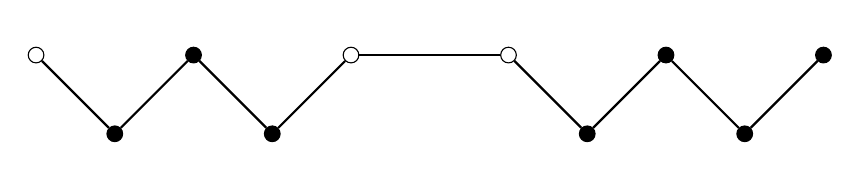
\begin{tikzpicture}[scale=1, auto,swap]
  
	
\node[draw,circle,inner sep=2pt] (01) at (0,1) {};
\node[draw,circle,inner sep=2pt,fill] (10) at (1,0) [label=below:]{};
\path[edge] (01) -- node[weight] {} (10);
\node[draw,circle,inner sep=2pt,fill] (21) at (2,1) [label=above:]{};
\path[edge] (21) -- node[weight] {} (10);
\node[draw,circle,inner sep=2pt,fill] (30) at (3,0) [label=below:]{};
\path[edge] (21) -- node[weight] {} (30);
\node[draw,circle,inner sep=2pt] (41) at (4,1) {};
\path[edge] (41) -- node[weight] {} (30);
\node[draw,circle,inner sep=2pt] (51) at (6,1) {};
\path[edge] (41) -- node[weight] {} (51);
\node[draw,circle,inner sep=2pt,fill] (70) at (7,0) [label=below:]{};
\path[edge] (51) -- node[weight] {} (70);
\node[draw,circle,inner sep=2pt,fill] (81) at (8,1) [label=above:]{};
\path[edge] (81) -- node[weight] {} (70);
\node[draw,circle,inner sep=2pt,fill] (90) at (9,0) [label=below:]{};
\path[edge] (81) -- node[weight] {} (90);
\node[draw,circle,inner sep=2pt,fill] (101) at (10,1) [label=above:]{};
\path[edge] (101) -- node[weight] {} (90);
\end{tikzpicture}

\caption{The gadget .}
\end{center}
\end{figure} 


The vertex  associated to clause , where , is
made adjacent to the vertices that correspond to the literals associated
with that clause. For example, if  we
will connect the vertex  with one of the vertices  and with one of the vertices . In order to make these
connections in a consistent way, we first fix an arbitrary ordering over the
clauses. If the variable  occurs as a positive literal in the clause , then we add the edge  of weight 3. Next, if 
 is the first clause that the variable  occurs with a negative
literal (in the fixed ordering of the clauses), then we add the edge  of weight 1. Finally, if the clause  is the
second clause that the variable  occurs as a negative literal, then
we add the edge  of weight 3. That is, if a
variable  appears only two times in , then only the two
distinguished vertices  and  of  are adjacent to a -vertex. This completes the
construction of the graph . Note that, by the construction of , in any
maximum greedy matching of , there are exactly four alternative ways to
match the edges of each of the subgraphs , as
illustrated in Fig.~\ref{fig:man}-\ref{fig:bad2}.




\subsection{APX-completeness\label{APX-subsec}} 
  
In order to prove that \greedy is APX-complete, first we prove in the next lemma that given an assignment that satisfies at least  
clauses we can construct a greedy matching with weight at least . 
The intuition for this lemma is as follows. Starting with a given satisfying 
truth assignment~ for the input formula~, we first construct the 
matching  in every  (cf.~Figure~\ref{fig:man}), and thus the
-vertices are initially free to be matched to -vertices. Then, if a 
variable  is true in , we change the matching of  from 
 to  (cf.~Figure~\ref{fig:map}), such that only the -vertex 
(and not the  and -vertices) of  is free to be 
matched to a -vertex. On the other hand, if the variable  is false in 
, then we either keep the matching  in , or we replace
 with  in  (cf.~Figure~\ref{fig:mann}). Note that in 
 only  is free to be matched, while in  both 
 and  are free to be matched with a -vertex; in 
both cases the -vertex of  is ``blocked'' from being 
matched to a -vertex. Then, using the fact that  satisfies at least  clauses 
of , we can construct a matching of~ where  -vertices are matched 
and the total weight of this matching is at least~.


\begin{lemma}
\label{lem:one}
If there is an assignment that satisfies at least  clauses then, there is a greedy 
matching with weight at least .
\end{lemma}

\begin{proof}
Given an assignment that satisfies  clauses we will construct a greedy 
matching of  with weight  by making use of the three matchings ,
, and  of , as illustrated in 
Figures~\ref{fig:man}-\ref{fig:map}. 
All these three matchings of  are greedy; furthermore note that
there also exists a fourth greedy matching \mbad of  
(see Fig.~\ref{fig:bad2}) which will not be used in the proof of the lemma. 




\begin{figure}[h!]
\begin{center}
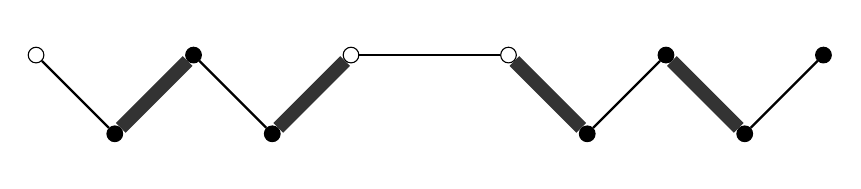
\begin{tikzpicture}[scale=1, auto,swap]
\node[draw,circle,inner sep=2pt] (01) at (0,1) {};
\node[draw,circle,inner sep=2pt,fill] (10) at (1,0) [label=below:]{};
\path[edge] (01) -- node[weight] {} (10);
\node[draw,circle,inner sep=2pt,fill] (21) at (2,1) [label=above:]{};
\path[matched] (21) -- node[weight] {} (10);
\node[draw,circle,inner sep=2pt,fill] (30) at (3,0) [label=below:]{};
\path[edge] (21) -- node[weight] {} (30);
\node[draw,circle,inner sep=2pt] (41) at (4,1) {};
\path[matched] (41) -- node[weight] {} (30);
\node[draw,circle,inner sep=2pt] (51) at (6,1) {};
\path[edge] (41) -- node[weight] {} (51);
\node[draw,circle,inner sep=2pt,fill] (70) at (7,0) [label=below:]{};
\path[matched] (51) -- node[weight] {} (70);
\node[draw,circle,inner sep=2pt,fill] (81) at (8,1) [label=above:]{};
\path[edge] (81) -- node[weight] {} (70);
\node[draw,circle,inner sep=2pt,fill] (90) at (9,0) [label=below:]{};
\path[matched] (81) -- node[weight] {} (90);
\node[draw,circle,inner sep=2pt,fill] (101) at (10,1)[label=above:] {};
\path[edge] (101) -- node[weight] {} (90);
\end{tikzpicture}
\caption{The matching  with weight 14 for the subgraph . 
For simplicity of notation we do not include the subscript  in the non-distinguished vertices.}
\label{fig:man}
\end{center}
\end{figure} 





\begin{figure}[h!]
\begin{center}
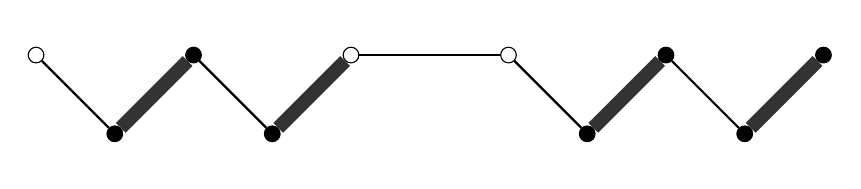
\begin{tikzpicture}[scale=1, auto,swap]
\node[draw,circle,inner sep=2pt] (01) at (0,1) {};
\node[draw,circle,inner sep=2pt,fill] (10) at (1,0) [label=below:]{};
\path[edge] (01) -- node[weight] {} (10);
\node[draw,circle,inner sep=2pt,fill] (21) at (2,1) [label=above:]{};
\path[matched] (21) -- node[weight] {} (10);
\node[draw,circle,inner sep=2pt,fill] (30) at (3,0) [label=below:]{};
\path[edge] (21) -- node[weight] {} (30);
\node[draw,circle,inner sep=2pt] (41) at (4,1) {};
\path[matched] (41) -- node[weight] {} (30);
\node[draw,circle,inner sep=2pt] (51) at (6,1) {};
\path[edge] (41) -- node[weight] {} (51);
\node[draw,circle,inner sep=2pt,fill] (70) at (7,0) [label=below:]{};
\path[edge] (51) -- node[weight] {} (70);
\node[draw,circle,inner sep=2pt,fill] (81) at (8,1) [label=above:]{};
\path[matched] (81) -- node[weight] {} (70);
\node[draw,circle,inner sep=2pt,fill] (90) at (9,0) [label=below:] {};
\path[edge] (81) -- node[weight] {} (90);
\node[draw,circle,inner sep=2pt,fill] (101) at (10,1) [label=above:]{};
\path[matched] (101) -- node[weight] {} (90);
\end{tikzpicture}
\caption{The matching  with weight 12 for the subgraph .}
\label{fig:mann}
\end{center}
\end{figure} 






\begin{figure}[h!]
\begin{center}
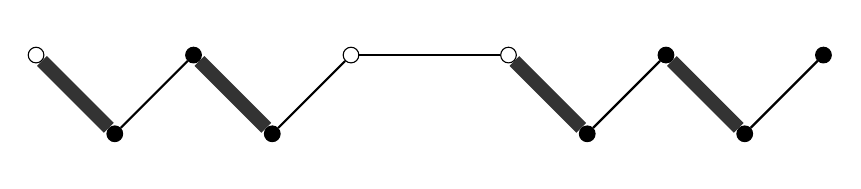
\begin{tikzpicture}[scale=1, auto,swap]
\node[draw,circle,inner sep=2pt] (01) at (0,1) {};
\node[draw,circle,inner sep=2pt,fill] (10) at (1,0) [label=below:]{};
\path[matched] (01) -- node[weight] {} (10);
\node[draw,circle,inner sep=2pt,fill] (21) at (2,1) [label=above:]{};
\path[edge] (21) -- node[weight] {} (10);
\node[draw,circle,inner sep=2pt,fill] (30) at (3,0) [label=below:]{};
\path[matched] (21) -- node[weight] {} (30);
\node[draw,circle,inner sep=2pt] (41) at (4,1) {};
\path[edge] (41) -- node[weight] {} (30);
\node[draw,circle,inner sep=2pt] (51) at (6,1) {};
\path[edge] (41) -- node[weight] {} (51);
\node[draw,circle,inner sep=2pt,fill] (70) at (7,0) [label=below:]{};
\path[matched] (51) -- node[weight] {} (70);
\node[draw,circle,inner sep=2pt,fill] (81) at (8,1) [label=above:]{};
\path[edge] (81) -- node[weight] {} (70);
\node[draw,circle,inner sep=2pt,fill] (90) at (9,0) [label=below:]{};
\path[matched] (81) -- node[weight] {} (90);
\node[draw,circle,inner sep=2pt,fill] (101) at (10,1) [label=above:]{};
\path[edge] (101) -- node[weight] {} (90);
\end{tikzpicture}
\caption{The matching  with weight 12 for the subgraph .}
\label{fig:map}
\end{center}
\end{figure} 





We construct the greedy matching of  with weight  as follows. 
Firstly, we set all the matchings for the subgraphs  to 
be the greedy matching , thus incurring a total weight of  from the 
currently matched edges. 
Then we process sequentially each clause  of the formula . 
If a clause  is satisfied in the given truth assignment by at least one 
\emph{positive} literal, then we choose one of these literals arbitrarily, say 
, and we change the matching of  to ; 
furthermore we match the edge  which has weight 3. 
In this case we replaced the matched edges  and 
 of  with total weight 7 by the matched 
edges , , and  
with total weight 8, i.e.~we increased the weight of the matching by 1. 



Assume that a clause  is satisfied in the given assignment only by 
\emph{negative} literals. 
If at least one of these literals of  corresponds to a -vertex, then
we match the edge  of weight 1. Thus in this case we also 
increase the total weight of the matched edges by 1. 
Finally, if all of these literals of  correspond to -vertices, then
we choose one of them arbitrarily, say , and we change the matching 
of  to ; furthermore we match the edge  
of weight 3. 
In this case we replaced the matched edges  and 
 of  with total weight 7 by the matched edges 
, , and  with total 
weight 8, i.e.~we increased the weight of the matching by 1. 
This completes the required matching  of the graph . 


Since we started with a matching of total weight  and we added weight 1 for
each of the  satisfied clauses in , note that the total weight of 
 is . 
In this matching , each of the induced subgraphs  of 
 is greedily matched. 
Furthermore all the remaining edges of  are edges that join a -vertex with
a distinguished vertex  (resp.~, ). 
Note that the weight of each of these edges is smaller than or equal to the 
weight of the edges adjacent to  (resp.~, )
within the subgraph . 
Thus, the matching  of  can be constructed greedily. Moreover, 
since  can be potentially further extended greedily to a matching 
with larger weight, it follows that the maximum greedy matching of  is at 
least .
\end{proof}

\medskip

Next we prove in Lemma~\ref{lem:at-least} that, if there is a greedy matching 
with weight , then there is an assignment that satisfies at least  
clauses.
In order to prove Lemma~\ref{lem:at-least}, first we prove in Lemma~\ref{lem:one-of-ag} a crucial property of the constructed graph , 
namely that in any greedy matching at most one of the vertices  and  can be matched with a -vertex.
\begin{lemma}
\label{lem:one-of-ag}
Let  be an arbitrary greedy matching of  and let 
. Then, in the subgraph , at most one of 
the vertices  and  can be matched with a -vertex.
\end{lemma}

\begin{proof}
The proof is done by contradiction. Assume otherwise that both  
and  are matched with some -vertices in . 
Note that both these edges that connect the vertices  and 
 with the corresponding -vertices have weight~3. Furthermore, 
none of the edges , , and 
 belong to . 
Thus, since the weight of the edge  is~4, it follows  is not greedy, which is a 
contradiction. 
That is, if both edges  and  of the subgraph
 are not matched within , then 
, as it is illustrated in the ``bad''
matching  of Fig.~\ref{fig:bad2}.
\end{proof}






\begin{figure}[h!]
\begin{center}
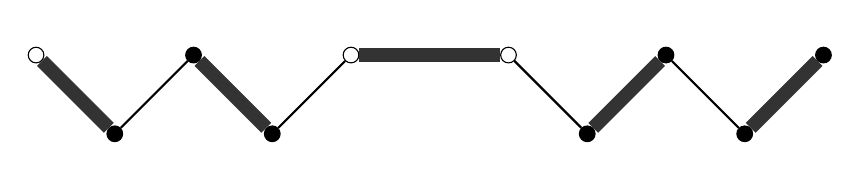
\begin{tikzpicture}[scale=1, auto,swap]
\node[draw,circle,inner sep=2pt] (01) at (0,1) {};
\node[draw,circle,inner sep=2pt,fill] (10) at (1,0) [label=below:]{};
\path[matched] (01) -- node[weight] {} (10);
\node[draw,circle,inner sep=2pt,fill] (21) at (2,1) [label=above:]{};
\path[edge] (21) -- node[weight] {} (10);
\node[draw,circle,inner sep=2pt,fill] (30) at (3,0) [label=below:]{};
\path[matched] (21) -- node[weight] {} (30);
\node[draw,circle,inner sep=2pt] (41) at (4,1) {};
\path[edge] (41) -- node[weight] {} (30);
\node[draw,circle,inner sep=2pt] (51) at (6,1) {};
\path[matched] (41) -- node[weight] {} (51);
\node[draw,circle,inner sep=2pt,fill] (70) at (7,0) [label=below:]{};
\path[edge] (51) -- node[weight] {} (70);
\node[draw,circle,inner sep=2pt,fill] (81) at (8,1) [label=above:]{};
\path[matched] (81) -- node[weight] {} (70);
\node[draw,circle,inner sep=2pt,fill] (90) at (9,0) [label=below:]{};
\path[edge] (81) -- node[weight] {} (90);
\node[draw,circle,inner sep=2pt,fill] (101) at (10,1) [label=above:] {};
\path[matched] (101) -- node[weight] {} (90);
\end{tikzpicture}
\caption{The ``bad'' matching \mbad for the subgraph  with weight 14.}
\label{fig:bad2}
\end{center}
\end{figure}






We are now ready to prove Lemma~\ref{lem:at-least}.

\begin{lemma}
\label{lem:at-least}
If there is a greedy matching with weight at least  in , then there exists 
an assignment that satisfies at least  clauses of the formula .
\end{lemma}

\begin{proof}
Let \mcal be a maximum weight greedy matching of  and assume that \mcal has 
weight at least . 
First we show that we can assume without loss of generality that, for every 
, the edges of the induced subgraph  are matched in \mcal 
according to one of the four matchings , , , and \mbad (see Figures~\ref{fig:man}-\ref{fig:bad2}). 
Assume that the edge  is matched in \mcal. 
Then clearly the edge  is also matched in \mcal, since this is the only valid greedy option for the right part of . 
Assume that the vertex  is matched in \mcal with a vertex different 
than . Then similarly the edges  and 
 are matched in \mcal. On the other hand, assume that the 
edge  is matched in \mcal. 
Then the edge  is also matched in \mcal due to the assumption
that \mcal is greedy.
Finally assume that the vertex  is matched in \mcal with a vertex
different than . 
Then, since \mcal is greedy, the edge  is matched in \mcal. 
Furthermore, since \mcal has the greatest weight among the greedy matchings of 
 by assumption, the vertex  is matched in \mcal either with 
vertex  or with its adjacent -vertex. 
If  is matched with the -vertex, then we replace this matched 
edge in \mcal by the matched edge  (if the vertex
 is unmatched) and we get an other greedy matching with the same weight. 
Therefore, we can assume without loss of generality that, for every , 
the edges of the induced subgraph  are matched in \mcal 
according to one of the four matchings , , , and \mbad, see 
Figures~\ref{fig:man}-\ref{fig:bad2}.



We construct from \mcal a truth assignment that satisfies at least  clauses 
of the formula , as follows. 
If the edges of the induced subgraph  are matched in \mcal according to one of the matchings  or , then we set the value of  to \emph{false}. 
If the edges of  are matched according to , then we set the value of  to \emph{true}. 
Otherwise, if the edges of  are matched according to \mbad, then set the truth value of  arbitrarily. 
Let now . Since the edges of the induced subgraph  are matched according to one of the matchings , , , and \mbad, as we proved above, 
it follows that the vertices  and  are not simultaneously matched with their associated -vertices in \mcal. 
Furthermore, Lemma~\ref{lem:one-of-ag} implies that at most one of the vertices 
 and  can be matched with their associated -vertices
in \mcal. 
Therefore the constructed truth assignment is valid.




Let . If  is matched according to \mbad in \mcal, then 
 clearly contributes weight 14 to the total weight of \mcal. 
Assume that  is matched according to  in \mcal, i.e.~assume 
that  is matched with a -vertex. 
Then  is matched with , and thus the right part of 
 (i.e.~the part between vertices  and ) 
contributes weight 7 to the total weight of \mcal. 
Furthermore the left part of  (i.e.~the part between vertices 
 and ) contributes weight 1+4+3=8 to the total weight
of \mcal. 
That is,  contributes weight 15 to the total weight of \mcal. 
Assume now that  is matched according to  or  in \mcal. 
If  is matched with  in \mcal, then the left part of 
contributes weight 3+4=7 to the total weight of \mcal. 
Otherwise, if  is matched with its adjacent -vertex in \mcal, 
then the left part of  contributes weight 1+3+4=8 to the total 
weight of \mcal. 
Similarly, if  is matched with  in \mcal, then the right 
part of  contributes weight 4+3=7 to the total weight of \mcal. 
Otherwise, if  is matched with its adjacent -vertex in \mcal, 
then the right part of  contributes weight 3+4+1=8 to the total 
weight of \mcal. 
Summarizing, if  of the vertices  are matched with -vertices in \mcal, then 
 contributes weight  to the total weight of \mcal. 



Therefore, since  has  induced subgraphs and the weight of \mcal is at 
least , it follows that  -vertices are matched in \mcal. 
For every vertex  that is matched with a vertex  in \mcal, 
the clause  contains the literal  and the variable  is set to 
true by the construction of the truth assignment. Thus  is satisfied. 
Similarly, for every vertex  that is matched with a vertex 
or  in \mcal, the clause  contains the literal  
and the variable  is set to false by the construction of the truth 
assignment. Thus  is again satisfied. 
Therefore, since  -vertices are matched in \mcal, it follows that
there are  satisfied clauses of  in the constructed assignment.
\end{proof}

\medskip

In the following theorem we conclude with the main result of this section.


\begin{theorem}
\label{thm:inai} \greedy is \emph{strongly NP-hard}
and \emph{APX-complete}. In particular, unless P=NP, \textsc{GreedyMatching}\xspace admits no PTAS, even on graphs with maximum degree at most 3 and with
at most three different integer weight values.
\end{theorem}

\begin{proof}
It follows by Lemmas~\ref{lem:one} and~\ref{lem:at-least} that there is a
greedy matching \mcal in  with weight at least  if
and only if there is a truth assignment that satisfies at least  clauses
in the 2SAT(3) formula . Thus it follows that \textsc{GreedyMatching} is NP-hard,
since MAX2SAT(3) is also NP-hard~\cite{Ausiello1999,RRR98}. Furthermore, since the graph  has three
different weight values (namely 1, 3, and 4), it follows that \textsc{GreedyMatching} is strongly NP-hard.

Denote by OPT the greatest number of clauses
that can be simultaneously satisfied by a truth assignment of .
Furthermore denote by OPT the maximum weight of a
greedy matching of the graph  that is constructed from  by our
reduction. Recall by construction that  has 3 different integer weights
and the maximum degree is 3. Then Lemma~\ref{lem:one} implies that OPTOPT. Note that a
random truth assignment satisfies each clause of  with probability , and thus there exists a truth assignment that satisfies at
least  clauses of , where  is the number of clauses,
and thus OPT. Since every
clause has at most 2 literals in , it follows that , and thus OPT.

Assume that there is a PTAS for computing OPT. Then for
every  we can compute in polynomial time a greedy matching  of  such that OPT. Given such a matching  we can compute by
Lemma \ref{lem:at-least} a truth assignment  of  such that . Therefore:

That is, assuming a PTAS for computing OPT, we obtain a
PTAS for computing OPT. This is a contradiction
by \cite{Ausiello1999}, unless P=NP. This proves that \textsc{GreedyMatching}\xspace is APX-hard. Furthermore \greedy clearly
belongs to the class APX, as any greedy matching algorithm achieves an -approximation for \greedy, and thus 
\greedy is APX-complete.
\end{proof}






















\subsection{Hardness of \greedy in Bipartite graphs
\label{hardness-bipartite-subsec}}

The graph  that we constructed from  (see Section~\ref {construction-subsec}) is not necessarily bipartite, as it may contain an
odd-length cycle. More specifically, it is possible that the following cycle
of length 9 exists: 

However, as we prove in this section, \greedy remains
strongly NP-hard also when the graph is in addition
bipartite.

To prove this (cf.~Theorem~\ref{thm:bip-hard}), we slightly modify our
reduction of Section~\ref{construction-subsec} and the proofs of Section \ref {APX-subsec}, as follows. We start with a 2-CNF formula , where every
variable appears in an \emph{arbitrary} number of clauses. We may assume
without loss of generality that every variable appears in  at least
three times; otherwise we may add dummy copies of existing clauses. Then we
create from  an equivalent 2-CNF formula  using a
technique of Papadimitriou and Yannakakis~\cite{PY91}. More specifically,
for every variable  that appears  times in , we
replace  by  new variables , one for
every clause of  in which  initially appeared. Furthermore
we add the  extra clauses , , , . Denote by  the resulting 2-CNF formula after
performing these operations for every . Note that in  a variable  occurs exactly in three clauses: two
times as  and one as  if  was
negative in , or two times as  and one as  if  was positive in . Furthermore, each
variable  occurs in one old clause from  and in two new
clauses in .

We will use again the gadgets  for each
variable  with a small modification. If the variable 
occurs two times in  as , then the
vertices  and  of  will correspond to the negative assignment of . Otherwise, if  occurs two times in  as a
positive literal, then the vertices  and  of  will correspond to the
positive assignment of . Again we will create one vertex 
for every clause  of . If the vertex 
corresponds to an old clause (i.e.~from the initial formula ) then we
connect it to the -vertices of the subgraphs  that correspond to these literals. If  corresponds to a
new clause in  then this clause is of the form . In this case we connect the corresponding -vertex with the vertex , if the variable 
occurs two times as a negative literal in , or with the
vertex , if  occurs two times as a positive
literal in . Similarly, the -vertex is connected with
the vertex , if the variable  occurs two
times as a negative literal in , or with , if  occurs two times as a positive literal in . The weights of these edges will be the same as before,
i.e.~each edge between a -vertex and a -vertex has weight 1 and
between a -vertex and an -vertex or a -vertex has
weight~3.

In order to prove that the constructed graph is bipartite, it is sufficient
to prove that there is no cycle with odd length. Let  be the set of all -vertices and of all -vertices and let  be the set
of all -vertices. First note that any cycle in the graph  must
contain at least two vertices from . Furthermore note that,
by the above construction, every path that connects two different vertices
of the set , without touching any vertex of the set , has even
length. Similarly, every path that connects two different vertices of the
set , without touching any vertex of the set , has also even
length. Thus every cycle in  that does not contain any vertex from  (resp.~from ) has even length. Consider now a cycle in  that
contains vertices from both sets  and . Then, if we traverse
this cycle in any direction, we will encounter the same number of transition
edges from set  to set  and from the set  to the set . Therefore the length of the cycle is even, and thus  is bipartite.
Thus, using the same argumentation as in Lemmas \ref{lem:one} and \ref {lem:at-least}, we obtain the following theorem.

\begin{theorem}
\label{thm:bip-hard} \greedy is strongly NP-hard,
even on \emph{bipartite} graphs with maximum degree at most 3 and with at
most three different integer weight values.
\end{theorem}




\subsection{Hardness results for \greedyv and \textsc{GreedyEdge}\xspace problems\label{hardness-additional-subsec}}

Having established the hardness results for \greedy in Sections~\ref{APX-subsec} and~\ref{hardness-bipartite-subsec}, we now
prove that also the decision problems \greedyv and 
\greedye are also strongly NP-hard.

\begin{theorem}
\label{thm:twohard} The decision problems \greedyv and 
\greedye are strongly NP-hard, even on
graphs with at most five different edge weights.
\end{theorem}

\begin{proof}
For the proof we amend the construction of Section~\ref{construction-subsec}
and the proofs of Section~\ref{APX-subsec}. Instead of reducing from the MAX2SAT(3) problem, 
we provide a reduction from the decision problem 3SAT(3). In this problem we are given a formula , 
in which every clause has at most 3 literals and every variable appears in at most 3 clauses, 
and the question is whether there exists a truth assignment that satisfies \emph{all clauses} of . 
This problem is NP-hard~\cite{Ausiello1999}. 


Let  be a 3SAT(3) formula with  variables and  clauses. We construct from  a weighted graph  in the same way as in Section~\ref{construction-subsec}, 
with the only difference that now every -vertex is connected to at most three (instead of at most two) distinguished vertices from the subgraphs . 
By following exactly the same proofs of Lemmas~\ref{lem:one} and~\ref{lem:at-least}, we can prove that this graph  has a greedy matching with weight at least  if and only if 
there exists a truth assignment that satisfies at least  clauses of the 3SAT(3) formula . 
Now we augment this graph  to a new graph  by adding two new vertices  and .
Vertex  is adjacent in  to all the -vertices of  with
edges of weight , while vertex  is adjacent in  only to vertex  with an edge of weight . Note
that  has five different edge weights.





Let  be a greedy matching in  and let  be the restriction of  on the edges of
the graph . Since every edge of  has larger weight than every edge
that is adjacent to  or to  in , it follows that  is also a greedy matching of . Assume that each of the  -vertices is matched in  with a vertex from the subgraphs . Then clearly . Conversely, assume that . If there
exists at least one vertex  that is not matched in  with
any vertex from a subgraph , then the edge  with weight  will be available to be matched in , and thus the edge  with weight  will not
belong to , a contradiction. Therefore,  if and only if each of the  -vertices is
matched in  a vertex from the subgraphs . Furthermore, it follows by the proofs of Lemmas~\ref{lem:one} and~\ref{lem:at-least} that each of the  -vertices is matched in  with a vertex from the subgraphs  if and only if
the weight of the greedy matching  of  is at least ,
or equivalently, if and only if there exists a truth assignment that
satisfies all  clauses of the formula .



Summarizing, there exists a greedy matching  of the
graph , in which the given edge  (resp.~the given
vertex ) is matched, if and only if the formula  is satisfiable. 
Thus, since 3SAT(3) is NP-hard, it follows that both decision problems \greedyv and \greedye 
are strongly NP-hard, even on graphs with at most five different edge weights.
\end{proof}


\section{Further natural parameters of \textsc{GreedyMatching}}

In this section we investigate the influence of two further natural parameters to the computational complexity of \greedy, 
other than the parameters maximum degree and number of different edge weights that we considered in Section~\ref{sec:hardness}. 
As the first parameter we consider in Section~\ref{ratio-subsec} the minimum ratio  
between two consecutive weight values, and as the second parameter we consider in Section~\ref{sec:param2} 
the maximum cardinality  of the connected components of , over all possible weight values . 
We prove that \greedy has a \emph{sharp threshold} behavior with respect to each of these parameters  and .

\subsection{Minimum ratio of consecutive weights\label{ratio-subsec}}

Here we consider the parameter , 
where  is the ratio between the th pair of consecutive edge weights. 
First we prove that, if , then there exists at least one 
maximum weight matching of  that is an optimum solution for \greedy on 
, obtaining the next theorem.

\begin{theorem}
\label{thm:rg2} \greedy can be computed in polynomial time if .
\end{theorem}

\begin{proof}
Let \mcal be a maximum weight matching for . Note that \mcal can be computed 
in polynomial time~\cite{Duan14}. Assume
that \mcal is not a greedy matching. We will construct from \mcal a greedy 
matching of  which has the same weight as \mcal, as follows. Since \mcal is 
not greedy, there must exist at least one edge  and two
incident edges ,
where each of the weights  and  of
the edges  and , respectively, is smaller
than the weight  of the edge . Since  and , it follows that , and thus . On the other hand , since \mcal is a
maximum weight matching by assumption. Therefore , and thus we can replace in \mcal the
edges  with the edge  without changing
the weight of \mcal.

We call all such edges  ``problematic''. Among
all problematic edges pick one edge  with the maximum weight and replace
its incident matched edges  with the edge 
in \mcal. We repeat this procedure until no problematic edge
is left, and thus we obtain a greedy matching  with
equal weight as \mcal. 
At each iteration the choice of the maximum weight problematic edge ensures
that no new problematic edges are created. We perform at most  iterations, and thus  is computed
in polynomial time.
\end{proof}

\medskip

Recall that in the proof of the Theorem~\ref{thm:inai} the weight values 1,
3, and 4 were used, thus the \greedy is hard for . In the next theorem we amplify this result by showing
that \greedy is NP-hard for any
constant . That is, complexity of \greedy has a threshold behavior at the parameter value .

\begin{theorem}
\label{thm:parlb} \greedy is \emph{strongly NP-hard} and \emph{APX-complete} 
for any constant , even on graphs with maximum degree at most 3 and with at most three different integer weight values.
\end{theorem}

\begin{proof}
For the proof we amend the weight values in the construction of Section~\ref{construction-subsec} 
and the proofs of Section~\ref{APX-subsec}. 
More specifically, in the construction of the graph  from the formula  
in Section~\ref{construction-subsec}, we replace each edge of weight 4 with
an edge of weight , and each edge of weight 3 with an edge of weight , 
where  is an arbitrary integer. In particular, the results of
Sections~\ref{construction-subsec} and~\ref{APX-subsec} are given for the value . 
By the proofs of Lemmas~\ref{lem:one} and~\ref{lem:at-least} 
(adapted for these new weights) it follows that there exists
a truth assignment that satisfies at least  clauses of the 2SAT(3)
formula  if and only if there is a greedy matching with weight at least  in the constructed graph . 
Similarly to Sections~\ref{construction-subsec} and~\ref{APX-subsec}, 
this graph  maximum maximum degree 3 and three different integer weight values. 
Furthermore,  can go arbitrarily close to 2 as  increases. 
The statement of the theorem follows exactly by the proof of Theorem~\ref{thm:inai}, adapted for these new weights of the edges of .
\end{proof}






\subsection{Maximum edge cardinality of a connected component in \label{sec:param2}}


Another parameter that we can consider is the maximum edge cardinality  of
the connected components of , among all different weights . 
Since  implies that there is a unique greedy matching for 
 which can be clearly computed in polynomial time, we consider the case .
In the original construction of Section~\ref{construction-subsec}, in every
gadget  there is a path with five edges where each edge
has weight 4. Thus  in the graph  of Section~\ref{construction-subsec}.
To prove our hardness result for  in Theorem \ref {thm-maximum-component-parameter}, we modify the gadgets  
as illustrated in Figure \ref{gadget-cardinality-parameter-fig}.
\begin{figure}[h]
\label{fig:modgx}
\par
\begin{center}
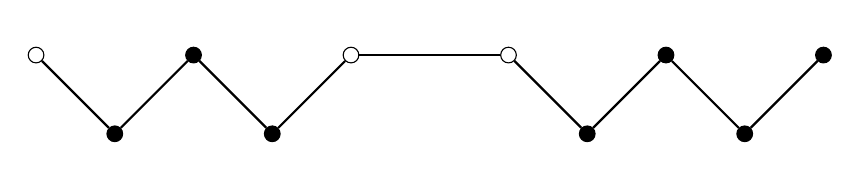
\begin{tikzpicture}[scale=1, auto,swap]
  
	
\node[draw,circle,inner sep=2pt] (01) at (0,1) {};
\node[draw,circle,inner sep=2pt,fill] (10) at (1,0) [label=below:]{};
\path[edge] (01) -- node[weight] {} (10);
\node[draw,circle,inner sep=2pt,fill] (21) at (2,1) [label=above:]{};
\path[edge] (21) -- node[weight] {} (10);
\node[draw,circle,inner sep=2pt,fill] (30) at (3,0) [label=below:]{};
\path[edge] (21) -- node[weight] {} (30);
\node[draw,circle,inner sep=2pt] (41) at (4,1) {};
\path[edge] (41) -- node[weight] {} (30);
\node[draw,circle,inner sep=2pt] (51) at (6,1) {};
\path[edge] (41) -- node[weight] {} (51);
\node[draw,circle,inner sep=2pt,fill] (70) at (7,0) [label=below:]{};
\path[edge] (51) -- node[weight] {} (70);
\node[draw,circle,inner sep=2pt,fill] (81) at (8,1) [label=above:]{};
\path[edge] (81) -- node[weight] {} (70);
\node[draw,circle,inner sep=2pt,fill] (90) at (9,0) [label=below:]{};
\path[edge] (81) -- node[weight] {} (90);
\node[draw,circle,inner sep=2pt,fill] (101) at (10,1) [label=above:]{};
\path[edge] (101) -- node[weight] {} (90);
\end{tikzpicture}
\end{center}
\par
\caption{The modified weights for the gadget .}
\label{gadget-cardinality-parameter-fig}
\end{figure}

Notice that in every subgraph  (see Figure~\ref {gadget-cardinality-parameter-fig}) the connected components of each weight
have edge cardinality at most 2. Furthermore, the weight of the edge between
a -vertex and a -vertex has weight 1, while the edges between 
a -vertex and an -vertex or a -vertex have weight~3. 
Thus these edges do not belong to any connected component with edges from 
. However, each -vertex is connected with at most
two distinguished vertices in different gadgets  and . Therefore  in the graph  of this
modified construction. Considering these updated gadgets  and using the same argumentation as in Lemmas~\ref{lem:one} and~\ref {lem:at-least}, we obtain that there is a greedy matching with weight at
least  in the constructed graph  if and only if there is a truth
assignment that satisfies at least  clauses from the original 2SAT(3)
formula , which implies the next theorem.

\begin{theorem}
\label{thm-maximum-component-parameter} 
\greedy is \emph{strongly NP-hard} and \emph{APX-complete} for ,
even on graphs with maximum degree at most 3 and with at most five different 
integer weight values.
\end{theorem}




\section{A randomized approximation algorithm\label{sec:approx}} 

In this section we provide a randomized approximation algorithm (\rgma) for \greedy with approximation ratio  on two special classes of graphs (cf.~Section~\ref{two-bush-subsec}). 
Furthermore we highlight an unexpected relation between \rgma and the randomized \mrg algorithm for greedily approximating the maximum cardinality matching (cf.~Section~\ref{bush-cardinality}), 
the exact approximation ratio of which is a long-standing open problem~\cite{PS12,ADFS95,DF91}. 
Before we present our randomized algorithm \rgma, we first introduce the following class of weighted graphs, called \emph{bush graphs}.



\begin{definition}[Bush graph]
\label{def:bushg}
An \emph{edge-weighted} graph  with  edge weight values  
is a \emph{bush graph} if, for every , the edges of  form a \emph{star}, 
which we call the \emph{-th bush} of .
\end{definition}




\begin{tcolorbox}[title=\rgma]
\textbf{Input:} Bush Graph  with edge weight values .\\
\textbf{Output:} A greedy matching \mrgma.\vspace{-2mm}
\begin{enumerate}
\item 
\vspace{-2mm}
\item \textbf{for}  \textbf{do}
\vspace{-2mm}
\item \hspace*{2mm} \textbf{if} 
\vspace{-2mm}
\item \hspace*{5mm} Select uniformly at random an edge  and add  to \mrgma
\vspace{-2mm}
\item \hspace*{5mm} Remove from  the endpoints of  and all edges of 
\end{enumerate}
\end{tcolorbox}




\subsection{Bush graphs and the maximum cardinality matching\label{bush-cardinality}}

In this section we present the connection of the problem \greedy on (weighted) bush graphs 
to the problem of approximating the maximum cardinality matching in unweighted graphs via randomized greedy algorithms, cf.~Theorem~\ref{thm:cardappx}. 
Notice that we cannot directly apply the \rgma algorithm on unweighted graphs, 
since the algorithm has to consider the different bushes in a specific total 
order which is imposed by the order of the weights. 
Thus, in order to approximate a maximum cardinality matching in a given unweighted graph  using the \rgma algorithm, 
we first appropriately convert  to a (weighted) bush graph  using the next Bush Decomposition algorithm, and then we apply \rgma on . 


\medskip

\begin{tcolorbox}[title= Bush Decomposition]
\textbf{Input:} Unweighted graph  and .\\
\textbf{Output:} A (weighted) bush graph .\vspace{-2mm}
\begin{enumerate}
\item Set 
\vspace{-2mm}
\item \textbf{while}  \textbf{do}
\vspace{-2mm}
\item \hspace*{2mm} Chose a random vertex  \label{gws3}
\vspace{-2mm}
\item \hspace*{2mm} For every  set 
\vspace{-2mm}
\item \hspace*{2mm} Remove the edges of  from 
\vspace{-2mm}
\item \hspace*{2mm} 
\end{enumerate}
\end{tcolorbox}

\medskip

Any unweighted graph  can be considered as a weighted graph with edge weights  for every edge , 
and thus in this case  coincides with the maximum cardinality matching in .
In the next lemma we relate  with .

\begin{lemma}
\label{lem:cardopt}
.
\end{lemma}
\begin{proof}
Assume that . Then, since the weight of each edge of  is 1 and the weight of each 
edge of  is by construction smaller than 1, it follows that  has strictly more edges than 
. This is a contradiction, since  is a maximum cardinality matching of . 
Therefore .


To prove that , we construct 
from a maximum cardinality matching \mcal of  
a maximum weight greedy matching  for  with the same cardinality as \mcal, 
i.e.~, as follows. 
Starting from , we sequentially visit all centers  
of the bushes in the weighted graph , in a decreasing order of their edge weights.
Whenever a center  of a bush in  is unmatched in , 
then all its neighbors must be matched. If one of these neighbors of  
is matched in the current matching with an edge that is lighter than the edges of the bush of , 
then we swap one of these edges with an edge incident to . 
That is, the only case where  stays unmatched is when all neighbors of  are matched 
with edges of larger weight in the current matching. In this case there exists a maximum
cardinality matching for  such that the vertex  is unmatched.
At the end we obtain a matching  with the same cardinality
as the initial matching , but now  is a greedy matching for 
. Thus, since  and the weight of  is 
, it follows that 
is less than or equal to the sum of the weight differences that have been 
introduced by ``Bush Decomposition'', i.e.~,
and thus .
\end{proof}



\medskip

With Lemma~\ref{lem:cardopt} in hand the next theorem follows:
\begin{theorem}
\label{thm:cardappx}
Let  be the approximation guarantee of \rgma algorithm on every bush graph. 
Then, for every , \rgma computes a -approximation of the 
maximum cardinality matching for unweighted graphs. 
\end{theorem}
We conjecture that a tight bound for  is ; in Section~\ref{two-bush-subsec} we prove our conjecture true for two subclasses of bush graphs. 
Note that, although vertex  in Step~\ref{gws3} of the Bush decomposition is selected at random, 
we do not use anywhere this fact in the proof of Lemma~\ref{lem:cardopt}. 
In particular, both Lemma~\ref{lem:cardopt} and Theorem~\ref{thm:cardappx} hold even when the choice of  in Step~\ref{gws3} is \emph{arbitrary}. 




\subsection{Randomized greedy matching in subclasses of bush graphs\label {two-bush-subsec}}

In this section we prove that our \textsc{Rgma}\xspace algorithm achieves an
approximation ratio  in two special classes of bush
graphs, cf.~Theorems~\ref{thm:app2bush} and~\ref{thm:appbush}. Before we
prove these two theorems we first need to prove the following three lemmas
which will be useful for our analysis.

\begin{lemma}
\label{claim0-lem} Let  be the center of the bush with the largest weight
in the graph . If the edge  belongs to a maximum greedy matching
of  then .
\end{lemma}

\begin{proof}
Let  be a maximum greedy matching of  that contains the
edge . Then  is a greedy matching of
the graph , and thus its weight is at most .
That is, ,
and thus .

Conversely, let now  be a maximum greedy matching of . Since  is the center of the bush with the largest weight in ,
it follows that every edge of  has weight less than . Therefore 
 is a greedy matching of , and
thus its weight is at most . That is, .
\end{proof}

\begin{lemma}
\label{claim1-1-lem}Let  be the largest edge weight  and let 
be a vertex . Then .
\end{lemma}

\begin{proof}
Let  be a maximum greedy matching of . If  is not matched
in  then , which satisfies
the statement of the lemma. Suppose now that  is matched in 
and let . We will modify the matching  of 
 to a matching  of  as follows. First remove
the edge  from  and let . If  is a greedy matching of 
then define ; note that in this case .
Otherwise, if  is not greedy,  must have either (a) a
neighbor  such that  is unmatched in  or (b) a neighbor  that is matched in  with an
edge , where . If  has both
such neighbors  and , we choose to consider only case
(a) if , or only case (b) if , breaking ties arbitrarily if . In case (a) we define ; then  is greedy and 


In case (b) we define . In this case 
If  is greedy then we define . Otherwise, if  is not greedy,  must have (similarly to the above) either (a) a neighbor  such that  is unmatched in  or (b) a neighbor  that is matched in  with an
edge , where . We continue to
update the matching  as above, until we reach a
matching  of  such that 
is greedy and . 
This completes the proof of the lemma, since  and .
\end{proof}

\medskip


In the next theorem we prove that \rgma achieves an approximation ratio of  when 
applied to a bush graph with only two different edge weights. 
Using this theorem as the induction basis, we then prove in Theorem~\ref{thm:app2bush} that 
\rgma achieves an approximation ratio of  also when applied to a bush graph in which every bush has at most two edges.

\begin{theorem}
\label{thm:app2bush}
\rgma is a -approximation when applied on bush graphs with only two
weights and with an arbitrary number of edges per bush.
\end{theorem}

\begin{proof}
Let  and  be the two bushes and let  be the center of the bush 
. We have to consider the following three cases:  is the center of the 
bush  too,  does not belong to the bush ,  is a leaf of the 
bush . 
If  is the center of the bush  too, then any greedy matching is 
consisted by only one edge from , thus \rgma always finds an optimal greedy
matching. 
When  does not belong to the bush  we can partition the edges of 
in three sets: 
\begin{itemize}
\item : edges of  that are incident to the center of the bush .
\item : edges of  that are not incident to leaves of .
\item : edges of  that are incident to a leaf of .
\end{itemize}
Without loss of generality we may assume that , since none 
of these edges can be chosen in any greedy matching. Furthermore, if 
, then \rgma will always choose one edge from the ,
thus it will return an optimal greedy matching. Finally, if , then 
for every choice of edge from , there will be at least one edge in  
that can be chosen in the greedy matching. Hence \rgma will construct an optimal
greedy matching. Finally suppose that  be the unique edge 
has. Then the probability that  is deleted in the first iteration of \rgma
is , thus \rgma will return a matching with expected weight 
. Hence the 
approximation guarantee of \rgma in this case is 
. 

Finally, we consider the case where  is a leaf of the bush . Then we 
may partition the edges of  into the following two sets:
\begin{itemize}
\item : edges of  that are adjacent only to one leaf of .
\item : edges of  that are adjacent to two leaves of .
\end{itemize}
If , then with probability  the 
algorithm returns a matching with weight . Thus, if this is the case
the approximation guarantee of the algorithm is at least . Hence,
without loss of generality we may assume that .  If 
, then the only case the algorithm \rgma returns a matching with
weight  is when the edge  is chosen; in every other case there
exists at least one in  that it is not deleted. This happens with 
probability . Notice that by our assumption it must be true 
that . Thus, the expected weight of the matching returned 
by the algorithm is . Hence the approximation guarantee of the \rgma 
is better than . The remaining case is when there is a unique edge 
. Then the \rgma returns a matching of weight  when at 
least one of the edges  and  is chosen in the first iteration. This 
happens with probability . Hence the expected weight of the 
matching returned by the algorithm is . Hence, in this case the 
approximation guarantee of the algorithm is at least .
\end{proof}

\medskip

We are now ready to prove the main theorem of this section.
\begin{theorem}
\label{thm:appbush} \textsc{Rgma}\xspace is a -approximation
when applied on bush graphs where each bush has at most two edges.
\end{theorem}

\begin{proof}
We will prove the claim by induction on the number of the different weight
values  the bush graph  has. We will use  to denote the expected weight of the greedy matching
produced by \textsc{Rgma}\xspace on the bush graph . We know from Theorem~\ref{thm:app2bush} that the claim holds when there are only two weight
values in . Assume that for any bush graph  with  different
weight values such that every bush of  has at most two edges, it holds
that . We
will prove that the claim holds also for bush graphs with  different
weight values.

Let  be the center of the bush with the largest weight  and
let  and  be the leaves of this bush. Without loss of
generality we can assume that all incident edges to  have weight , since every other incident edge of  with weight 
would never be selected by the greedy algorithm. Assume that the edge  belongs to the optimal greedy matching of . Thus,  by
Lemma \ref{claim0-lem}. Furthermore  by Lemma \ref{claim1-1-lem}. Hence we get 
Now note that 
and  by Lemma~\ref{claim1-1-lem}. 
Therefore , and thus

\end{proof}




\begin{comment}
\paragraph{\bf .}
Let  be the weight values of the bush graph. We can 
write the bush graph as  where  is the center of the bush of weight 
 and and  is a bush graph with  different weight values. Furthermore,
let  be the set of vertices that are the leaves 
of the bush . Clearly, every greedy matching will have an edge  
where . 

The expected weight  of the greedy matching produced by \rgma on the
bush graph  is

Furthermore, it holds that , thus . Combining that with the Equation~\ref{eq:avg} we get that

\end{comment}



\section{Conclusions}

Several interesting open questions stem from our paper. 
Probably the most important one is to derive tight approximation guarantees 
 for the maximum weight greedy matching problem, even for bush graphs. 
We conjecture that ; an affirmative answer to our conjecture 
would imply that the algorithm \mrg for maximum cardinality matching in 
unweighted graphs has an approximation ratio of almost , thus 
solving a longstanding open problem~\cite{PS12,ADFS95,DF91}. We believe that our
approach might provide novel ways of better analysis of the \mrg algorithm.
As we proved, \greedy is NP-hard even on graphs of maximum degree three with at 
most three different weight values on their edges. It remains open whether \greedy can be solved 
efficiently when there are only two weight values on the edges of the input graph.



{\small 
\begin{thebibliography}{10}

\bibitem{ABS07}
D.~Abraham, A.~Blum, and T.~Sandholm.
\newblock Clearing algorithms for barter exchange markets: enabling nationwide
  kidney exchanges.
\newblock In {\em Proceedings 8th {ACM} Conference on Electronic Commerce
  ({EC})}, pages 295--304, 2007.

\bibitem{AIKM}
D.~Abraham, R.~Irving, T.~Kavitha, and K.~Mehlhorn.
\newblock Popular matchings.
\newblock {\em SIAM Journal on Computing}, 37(4):1030--1045, 2007.

\bibitem{ABH13}
E.~Anshelevich, O.~Bhardwaj, and M.~Hoefer.
\newblock Friendship and stable matching.
\newblock In {\em Algorithms - {ESA} 2013 - 21st Annual European Symposium,
  Sophia Antipolis, France, September 2-4, 2013. Proceedings}, pages 49--60,
  2013.

\bibitem{ADN13}
E.~Anshelevich, S.~Das, and Y.~Naamad.
\newblock Anarchy, stability, and utopia: creating better matchings.
\newblock {\em Autonomous Agents and Multi-Agent Systems}, 26(1):120--140,
  2013.

\bibitem{ADFS95}
J.~Aronson, M.~Dyer, A.~Frieze, and S.~Suen.
\newblock Randomized greedy matching {II}.
\newblock {\em Random Structures \& Algorithms}, 6(1):55--73, 1995.

\bibitem{Ausiello1999}
G.~Ausiello, M.~Protasi, A.~Marchetti-Spaccamela, G.~Gambosi, P.~Crescenzi, and
  V.~Kann.
\newblock {\em Complexity and Approximation: Combinatorial Optimization
  Problems and Their Approximability Properties}.
\newblock Springer-Verlag, 1999.

\bibitem{Avis83}
D.~Avis.
\newblock A survey of heuristics for the weighted matching problem.
\newblock {\em Networks}, 13(4):475--493, 1983.

\bibitem{Duan14}
R.~Duan and S.~Pettie.
\newblock Linear-time approximation for maximum weight matching.
\newblock {\em Journal of the ACM}, 61(1):1--23, 2014.

\bibitem{DF91}
M.~Dyer and A.~Frieze.
\newblock Randomized greedy matching.
\newblock {\em Random Structures \& Algorithms}, 2(1):29--45, 1991.

\bibitem{DFP93}
M.~Dyer, A.~Frieze, and B.~Pittel.
\newblock The average performance of the greedy matching algorithm.
\newblock {\em Annals of Applied Probability}, 3(2):526--552, 05 1993.

\bibitem{Edmonds}
J.~Edmonds.
\newblock {\em Classic Papers in Combinatorics}, chapter Paths, Trees, and
  Flowers, pages 361--379.
\newblock Birkh{\"a}user Boston, Boston, MA, 1987.

\bibitem{FL10}
D.~R. Ford and D.~R. Fulkerson.
\newblock {\em Flows in Networks}.
\newblock Princeton University Press, 2010.

\bibitem{HK78}
D.~Hausmann and B.~Korte.
\newblock K-greedy algorithms for independence systems.
\newblock {\em Zeitschrift f{\"u}r Operations Research}, 22(1):219--228, 1978.

\bibitem{J79}
B.~Jovanovic.
\newblock Job matching and the theory of turnover.
\newblock {\em Journal of Political Economy}, 87(5):972--990, 1979.

\bibitem{MP97}
Z.~Miller and D.~Pritikin.
\newblock On randomized greedy matchings.
\newblock {\em Random Structures \& Algorithms}, 10(3):353--383, 1997.

\bibitem{PY91}
C.~Papadimitriou and M.~Yannakakis.
\newblock Optimization, approximation, and complexity classes.
\newblock {\em Journal of Computer and System Sciences}, 43(3):425--440, 1991.

\bibitem{PS12}
M.~Poloczek and M.~Szegedy.
\newblock Randomized greedy algorithms for the maximum matching problem with
  new analysis.
\newblock In {\em Proceedings of the 53rd Annual {IEEE} Symposium on
  Foundations of Computer Science ({FOCS})}, pages 708--717, 2012.

\bibitem{RRR98}
V.~Raman, B.~Ravikumar, and S.~S. Rao.
\newblock A simplified {NP}-complete {MAXSAT} problem.
\newblock {\em Information Processing Letters}, 65(1):1--6, 1998.

\bibitem{R84}
A.~Roth.
\newblock The evolution of the labor market for medical interns and residents:
  {A} case study in game theory.
\newblock {\em Journal of Political Economy}, 92(6):991--1016, 1984.

\bibitem{RP99}
A.~Roth and E.~Peranson.
\newblock {The redesign of the matching market for American physicians: Some
  engineering aspects of economic design}.
\newblock Technical report, NBER Working Papers 6963, 1999.

\bibitem{R04}
A.~Roth, T.~S\"onmez, and M.~\"Unver.
\newblock Kidney exchange.
\newblock {\em The Quarterly Journal of Economics}, 119(2):457--488, 2004.

\bibitem{San09}
P.~Sankowski.
\newblock Maximum weight bipartite matching in matrix multiplication time.
\newblock {\em Theoretical Computer Science}, 410(44):4480 -- 4488, 2009.

\end{thebibliography}
}



\end{document}
